% ===== main.tex (CORRECTED & UPGRADED) =====
\documentclass[12pt, letterpaper, onecolumn]{report}

% --- CORE PACKAGES ---
\usepackage[margin=1in]{geometry}
\usepackage{amsmath, amssymb, amsthm, mathtools} % <-- CORRECTED THIS LINE
\usepackage{graphicx}
\usepackage{setspace}
\usepackage{url}
\usepackage{booktabs}
\usepackage{longtable}
\usepackage{tikz}
\usetikzlibrary{arrows.meta, positioning, decorations.pathmorphing, shapes.geometric, calc}
\usepackage[authoryear]{natbib}
\usepackage[colorlinks=true, allcolors=blue]{hyperref}
\usepackage{pgfplots}
\pgfplotsset{compat=1.18}
\usepackage{subcaption}
\usepackage[nameinlink,capitalize]{cleveref} % Loaded for smart referencing
\usepackage{nomencl}
\makenomenclature

% --- STYLING ---
\onehalfspacing
\setcounter{tocdepth}{3} % Show subsubsections in ToC
\urlstyle{same} 

% --- THEOREM ENVIRONMENTS (CORRECTED) ---
\theoremstyle{plain}
\newtheorem{theorem}{Theorem}[chapter]
\newtheorem{proposition}[theorem]{Proposition} % Shares counter with theorem
\newtheorem{lemma}[theorem]{Lemma}             % Shares counter with theorem
\newtheorem{corollary}[theorem]{Corollary}       % Shares counter with theorem
\theoremstyle{definition}
\newtheorem{definition}[theorem]{Definition}     % Shares counter with theorem
\newtheorem{assumption}[theorem]{Assumption}     % Shares counter with theorem
\theoremstyle{remark}
\newtheorem{remark}[theorem]{Remark}             % Shares counter with theorem


% --- CUSTOM COMMANDS ---
\newcommand{\E}{\mathbb{E}}
\newcommand{\R}{\mathbb{R}}
\newcommand{\D}{\mathcal{D}}
\newcommand{\A}{\mathcal{A}}
\newcommand{\N}{\mathcal{N}}
\newcommand{\Eff}{\mathcal{E}}
\newcommand{\Nov}{\mathcal{N}}
\newcommand{\Hc}{H_c}
\newcommand{\alg}{\mathcal{A}}
\newcommand{\I}{\mathcal{I}}

% --- TITLE PAGE INFORMATION ---
\title{
    \vspace{1in}
    \textbf{Emergent Machine Pedagogy: \\ A Game-Theoretic Framework for Autonomous Teaching} \\
    
}
\author{Mohana Rangan Desigan}
\date{August 17, 2025}

% --- DOCUMENT START ---
\begin{document}

\maketitle
\cleardoublepage

% --- FRONT MATTER ---
\pagenumbering{roman}

\chapter*{Abstract}
\addcontentsline{toc}{chapter}{Abstract}
\noindent The dominant paradigm for AI tutoring is imitation learning. While successful, this approach is fundamentally constrained by a theoretical ceiling on its inventive capacity. This thesis proposes a new paradigm: \textbf{Pedagogy as a Self-Discovering Game}. We argue that inventive teaching strategies can emerge from the interactions of autonomous agents within a principled, game-theoretic framework, analogous to how self-play unlocked superhuman strategies in games.

We formalize this paradigm by introducing the COGNITA stochastic game. Our theoretical contributions form a comprehensive framework that establishes this as a new, robust field of inquiry. We prove the \textbf{Imitation Efficacy Ceiling}, an impossibility theorem on imitation. We then prove a \textbf{Discovery-Efficacy Tradeoff Theorem}, establishing the mathematical license for our system to invent novel strategies that exceed this ceiling, connecting it to principles of information bottleneck theory. We theorize a \textbf{Critical Diversity Threshold}, a phase transition where emergent curricula appear, linking our AI system to established models in cognitive science from Piaget and Vygotsky. We provide a \textbf{PAC-Verifier Guarantee} that serves as a formal alignment guarantee for the system's safety and reliability. Finally, we prove a \textbf{No Free Lunch for Pedagogy Theorem}, showing that invention is provably impossible without the core components of our system.

To validate this theory, we propose a series of computationally feasible experiments. Using a custom-built Self-Structuring Cognitive Agent (SSCA) as a computational model of pedagogy, we will provide the first empirical evidence of a system breaking the imitation ceiling. Each experiment is designed as the explicit empirical analogue of a corresponding theorem. This work aims to shift the frontier of AI research from building systems that retrieve knowledge to creating systems that can autonomously discover and structure the principles of pedagogy, with profound implications for cognitive science, education, and AI safety.
\cleardoublepage

\chapter*{Acknowledgments}
\addcontentsline{toc}{chapter}{Acknowledgments}
% ===== chapters/00-acknowledgments.tex =====

% First and foremost, I extend my deepest gratitude to my advisor, [Advisor's Name], whose guidance was the bedrock of this research. Your intellectual generosity, incisive feedback, and unwavering support transformed nascent ideas into a coherent framework. This dissertation would not exist without your mentorship.

% I am also indebted to the members of my thesis committee, [Committee Member 1's Name] and [Committee Member 2's Name], for their invaluable insights and challenging questions, which sharpened this work immeasurably.

% My time at [Your Research Group/Lab] has been a remarkable journey, and I thank my colleagues and friends for the countless stimulating discussions, whiteboard sessions, and shared moments of discovery and frustration. In particular, I thank [Colleague's Name] for [Specific contribution, e.g., "the late-night brainstorming that led to the formulation of the PAC-Verifier guarantee"] and [Another Colleague's Name] for their constant encouragement.

% This research was generously supported by [Funding Source, e.g., "the National Science Foundation Graduate Research Fellowship Program under Grant No. XXXXX"].

% Finally, to my family—my parents, [Parents' Names], and my partner, [Partner's Name]—thank you for your endless love, patience, and belief in me. Your support has been my foundation.
\cleardoublepage

\tableofcontents
\cleardoublepage
\listoffigures
\addcontentsline{toc}{chapter}{List of Figures}
\cleardoublepage
\listoftables
\addcontentsline{toc}{chapter}{List of Tables}
\cleardoublepage

% --- MAIN MATTER ---
\pagenumbering{arabic}

\chapter{Introduction: A New Paradigm for Machine Pedagogy}

\section{The Imitation Ceiling}
The modern era of Artificial Intelligence is largely defined by the success of imitation learning. However, this success masks a fundamental limitation: an imitative system is a high-fidelity mirror, but a mirror cannot create a new image. In education, this translates to an \textbf{Imitation Efficacy Ceiling}. An AI tutor trained on a dataset of human teaching examples can learn to be as effective as the best teacher in that dataset, but it can never systematically surpass them. This thesis argues that to create truly intelligent pedagogical agents, we must move beyond imitation.

\section{Thesis Statement: Pedagogy as a Self-Discovering Game}
This dissertation introduces and validates a new paradigm for artificial intelligence: \textbf{Pedagogy as a Self-Discovering Game}. We posit that inventive, effective, and robust pedagogical strategies can emerge from the co-evolutionary dynamics of autonomous agents operating within a principled, game-theoretic framework. We position this work alongside foundational shifts in AI research, such as Self-Play in Reinforcement Learning \citep{silver2017mastering}. Just as self-play unlocked superhuman strategic gameplay, we propose that a principled "self-teaching" game can unlock the discovery of superhuman pedagogy.

\section{Core Contributions}
This thesis will make four primary contributions, composed of a rigorous theoretical framework and a series of monumental, yet computationally feasible, experiments designed to validate it.

\begin{enumerate}
    \item \textbf{A New Theoretical Quintet for Emergent Pedagogy:} We provide a chain of five theorems that establish the foundations of our paradigm: an impossibility theorem for imitation, a possibility theorem for discovery, a phase transition theorem for invention, a robustness theorem for alignment, and a necessity theorem proving no free lunch.
    \item \textbf{The Self-Structuring Cognitive Agent (SSCA):} We design and implement a novel agent architecture that serves as a computational model of human pedagogy, learning not only a teaching policy but also simultaneously building an internal, dynamic "world model" of the conceptual space it is teaching.
    \item \textbf{The First Empirical Demonstration of Breaking the Imitation Ceiling:} We will conduct a series of experiments, feasible on a free-tier cloud budget, that provide the first clear, statistically significant evidence of an AI system discovering pedagogical strategies superior to those in its initial expert dataset.
    \item \textbf{A Tightly-Coupled Theoretical-Empirical Loop:} Each experiment is explicitly designed as the empirical analogue of a core theorem, creating a closed, unassailable argument that bridges formal theory and empirical validation.
\end{enumerate}
% ===== chapters/02-theory.tex (UPGRADED with Formal Preliminaries) =====
\chapter{A Theoretical Quintet for Emergent Pedagogy}
\label{chap:theory}

Our theoretical framework is built upon the COGNITA stochastic game formalism. It provides a quintet of theorems that creates a complete intellectual arc: defining the limits of the old paradigm (impossibility), proving the potential of the new (possibility), describing the mechanism of discovery (phase transition), guaranteeing its stability and alignment (robustness), and proving its components are essential (necessity).

% ===================================================================
% ===== NEW SECTION: FORMAL PRELIMINARIES (Phase 1, Step 1.1) =====
% ===================================================================
\section{Formal Preliminaries and Assumptions}
\label{sec:preliminaries}

Before presenting our main theorems, we establish the mathematical groundwork. A rigorous formulation requires precise definitions of the spaces and functions governing agent interaction, as well as the explicit assumptions that guarantee well-behaved learning dynamics.

\paragraph{Spaces and Functions.}
Let $\mathcal{L}$ be the space of all possible natural language strings.
\begin{itemize}
    \item \textbf{Policy Space ($\Pi_i$):} For each agent $i \in N$, a policy $\pi_i$ is a mapping from a state $s \in \mathcal{S}$ to a probability distribution over its action space $\mathcal{A}_i \subset \mathcal{L}$. We define the policy space $\Pi_i$ as the set of all such valid policies for agent $i$. A joint policy is denoted by $\pi = (\pi_i)_{i \in N} \in \Pi = \prod_{i \in N} \Pi_i$.
    
    \item \textbf{Pedagogical Efficacy ($\Eff$):} We define a central function, Pedagogical Efficacy $\Eff: \Pi \to [0, 1]$, which measures the success of a joint policy. It is the expected, discounted reward of the Student agent $\mathbb{S}$ under that policy:
    \[
    \Eff(\pi) \coloneqq \E_{\pi} \left[ \sum_{t=0}^{\infty} \gamma^t R_{\mathbb{S}}(s_t, a_t) \mid s_0 \right]
    \]
    where the expectation is taken over the trajectories of states and actions induced by the joint policy $\pi$.
    
    \item \textbf{Population Diversity ($D$):} Let $\mathcal{P}(\Pi_{\mathbb{T}})$ be a probability distribution over the Teacher's policy space, representing a population of teaching strategies. We define the diversity of this population, $D: \mathcal{P}(\Pi_{\mathbb{T}}) \to \R^+$, as the Shannon entropy of the distribution. For a discrete set of policies $\{\pi^{(j)}\}$ with probabilities $\{p_j\}$, this is:
    \[
    D(\{\pi^{(j)}\}) = -\sum_j p_j \log p_j
    \]
\end{itemize}

\paragraph{Foundational Assumptions.}
Our framework relies on standard assumptions from game theory and reinforcement learning to ensure the existence and stability of equilibria.

\begin{assumption}[Compactness and Convexity]
\label{assump:compactness}
For each agent $i \in N$, the policy space $\Pi_i$ is a compact and convex subset of a locally convex topological vector space.
\end{assumption}

\begin{assumption}[Continuity of Payoffs]
\label{assump:continuity}
For each agent $i \in N$, the expected payoff function $J_i(\pi) = \E_{\pi}[\sum \gamma^t R_i]$ is continuous in the joint policy $\pi$.
\end{assumption}

\begin{remark}[Guaranteeing Equilibrium]
\Cref{assump:compactness} and \Cref{assump:continuity} satisfy the preconditions for Glicksberg's fixed-point theorem \citep{glicksberg1952further}, a generalization of Nash's existence theorem to infinite games. This guarantees that the COGNITA game admits at least one Stationary Nash Equilibrium (SNE).
\end{remark}

\begin{assumption}[Contraction Mapping]
\label{assump:contraction}
Let $BR(\pi) = (BR_i(\pi_{-i}))_{i \in N}$ be the joint best-response correspondence. We assume there exists a metric on the joint policy space $\Pi$ such that the best-response dynamic is a contraction mapping with modulus $k \in [0, 1)$. That is, for any two joint policies $\pi, \pi' \in \Pi$:
\[
d(BR(\pi), BR(\pi')) \le k \cdot d(\pi, \pi')
\]
\end{assumption}

\begin{remark}[Uniqueness and Stability]
By the Banach Fixed-Point Theorem, \Cref{assump:contraction} guarantees that the Nash Equilibrium is unique and that iterative learning dynamics (such as fictitious play or evolutionary strategies) will converge to this unique equilibrium. This ensures our learning process is stable and predictable.
\end{remark}
% ===================================================================
% ===== END OF NEW SECTION ==========================================
% ===================================================================

\section{The COGNITA Stochastic Game Formalism}

We now formally define our paradigm. The \emph{COGNITA Stochastic Game}, built upon the preliminaries in \Cref{sec:preliminaries}, provides the foundation for our theorems.

\begin{figure}[htbp]
\centering
\begin{tikzpicture}[node distance=2.2cm, >=Latex]
\node[draw, rounded corners, thick, align=center, minimum width=3.0cm, minimum height=1.1cm] (S) {$s=(\tau,h,z)$\\ \small state};
\node[draw, rounded corners, thick, above left=of S] (T) {Teacher $\mathbb{T}$};
\node[draw, rounded corners, thick, below left=of S] (St) {Student $\mathbb{S}$};
\node[draw, rounded corners, thick, above right=of S] (C) {Curriculum $\mathbb{C}$};
\node[draw, rounded corners, thick, below right=of S] (V) {Verifier $\mathbb{V}$};

\draw[->, thick] (T) -- node[above left]{hint $a_{\mathbb{T}}$} (S);
\draw[->, thick] (St) -- node[below left]{solution $a_{\mathbb{S}}$} (S);
\draw[->, thick] (C) -- node[above right]{task $a_{\mathbb{C}}$} (S);
\draw[->, thick] (V) -- node[below right]{grade $a_{\mathbb{V}}$} (S);

\draw[->, thick, bend left=12] (S) to node[above]{\small $\mathcal{T}(s,a)\to s'$} +(3.8,0) to[bend left=12] node[below]{\small rewards $R_i$} (S);
\end{tikzpicture}
\caption{The COGNITA stochastic game: four agents interact through language actions with state transitions $\mathcal{T}$ and rewards $R_i$.}
\label{fig:schematic}
\end{figure}

\begin{definition}[The COGNITA Stochastic Game]
A pedagogical stochastic game is a tuple
\[
\mathcal{G} = \langle N, \mathcal{S}, \{\mathcal{A}_i\}_{i \in N}, \mathcal{T}, \{R_i\}_{i \in N}, \gamma \rangle
\]
with the following components:
\begin{itemize}
    \item \textbf{Agents:} $N = \{\mathbb{T}, \mathbb{S}, \mathbb{C}, \mathbb{V}\}$,
    corresponding to a \emph{Teacher}, \emph{Student}, \emph{Curriculum Generator},
    and \emph{Verifier}.
    \item \textbf{State Space:} $\mathcal{S}$ is the set of states. A state $s \in \mathcal{S}$
    is represented as $s = (\tau, h, z)$ where $\tau$ is the current task,
    $h$ is the dialogue history, and $z$ is the latent representation of the Student's conceptual knowledge. This state $z$ is a computational analogue of the cognitive structures in Piaget's theory of equilibration \citep{piaget1977equilibration} and the "zone of proximal development" in Vygotsky's work \citep{vygotsky1978mind}.
    \item \textbf{Action Spaces:}
    For each agent $i \in N$, the set of actions $\mathcal{A}_i$ is a compact metric space of natural language strings.
    \item \textbf{Transition Function:}
    $\mathcal{T}: \mathcal{S} \times \prod_{i \in N}\mathcal{A}_i \to \Delta(\mathcal{S})$
    is a Markovian transition kernel governing the state dynamics.
    \item \textbf{Reward Functions:}
    For each agent $i \in N$, the bounded payoff
    $R_i: \mathcal{S} \times \prod_{i \in N}\mathcal{A}_i \to [0,1]$. For instance, $R_{\mathbb{T}}$ is high when the student succeeds with concise, effective hints, framing teaching as an optimization problem of maximizing information transfer under a complexity constraint, akin to the information bottleneck principle \citep{tishby2000information}.
    \item \textbf{Discount Factor:}
    $\gamma \in [0,1)$ discounts future payoffs.
\end{itemize}
\end{definition}

Our foundational assumptions (\Cref{assump:compactness,assump:continuity,assump:contraction}) ensure that the learning process within this game is well-behaved and converges to a unique, stable equilibrium.

\section{The Quintet}

\subsection{Impossibility: The Imitation Efficacy Ceiling}
\paragraph{Intuition.} This theorem formalizes the core limitation of imitation learning. By restricting an agent to the convex hull of expert demonstrations, we inherently limit its expressive capacity. It can interpolate between known good strategies, but it cannot extrapolate to discover a truly novel strategy that lies outside this hull. Its performance is therefore forever capped by the best-performing expert in its original dataset.

\begin{theorem}[Imitation Efficacy Ceiling]
\label{thm:imitation_ceiling}
Let the Teacher's policy space $\Pi_{\mathbb{T}}$ be restricted to the convex hull of a finite set of expert policies $\{\pi^{(j)}\}_{j=1}^k$. Let $\eta = \max_{j \in \{1,..,k\}} \Eff(\pi^{(j)})$ be the efficacy of the best expert policy. Then for any policy $\pi \in \Pi_{\mathbb{T}}$, its efficacy is bounded: $\Eff(\pi) \le \eta$.
\end{theorem}
\begin{proof}
The proof proceeds by first establishing the linearity of the efficacy function with respect to policy mixtures and then applying the definition of the maximum.

\noindent\textbf{1. Expressing the Mixed Policy.} By the definition of the convex hull, any policy $\pi \in \Pi_{\mathbb{T}}$ can be expressed as a convex combination of the expert policies,
\[
\pi = \sum_{j=1}^k \alpha_j \pi^{(j)}
\]
where the coefficients $\alpha_j \ge 0$ for all $j=1, \dots, k$ and $\sum_{j=1}^k \alpha_j = 1$. A sample from this mixed policy $\pi(a|s)$ is generated by first sampling an index $j$ from the categorical distribution defined by the weights $\{\alpha_j\}$, and then sampling an action $a$ from the chosen expert policy $\pi^{(j)}(a|s)$.

\noindent\textbf{2. Linearity of the Efficacy Function.} Recall the definition of efficacy from \Cref{sec:preliminaries}: $\Eff(\pi) = \E_{\pi} [ \sum_{t=0}^{\infty} \gamma^t R_{\mathbb{S}}(s_t, a_t) ]$. The expectation $\E_{\pi}$ is taken over trajectories generated by the mixed policy $\pi$. We can decompose this expectation using the law of total expectation, conditioning on the choice of the underlying expert policy at each step. Because the choice of expert $j$ is made independently at each step according to the fixed weights $\{\alpha_j\}$, the trajectory distribution induced by $\pi$ is equivalent to a mixture of the trajectory distributions induced by each $\pi^{(j)}$. Therefore, the expectation is linear in the mixture components:
\[
\Eff(\pi) = \Eff\left(\sum_{j=1}^k \alpha_j \pi^{(j)}\right) = \sum_{j=1}^k \alpha_j \Eff(\pi^{(j)})
\]

\noindent\textbf{3. Applying the Bound.} By definition, $\eta$ is the maximum efficacy achieved by any expert policy. Thus, for any individual expert policy $\pi^{(j)}$, we have:
\[
\Eff(\pi^{(j)}) \le \eta \quad \forall j \in \{1, \dots, k\}
\]
Substituting this inequality into our linear expansion of $\Eff(\pi)$:
\[
\Eff(\pi) = \sum_{j=1}^k \alpha_j \Eff(\pi^{(j)}) \le \sum_{j=1}^k \alpha_j \eta
\]

\noindent\textbf{4. Conclusion.} Since $\eta$ is a constant, we can factor it out of the summation. Using the property that the weights of a convex combination sum to unity:
\[
\Eff(\pi) \le \eta \sum_{j=1}^k \alpha_j = \eta \cdot 1 = \eta
\]
Thus, we have shown that $\Eff(\pi) \le \eta$. This establishes that no policy confined to the convex hull of the expert set can exceed the performance of the single best expert policy within that set.
\end{proof}

\subsection{Possibility: The Discovery-Efficacy Tradeoff}
\paragraph{Intuition.} To break the imitation ceiling, an agent must explore. However, exploration is inherently risky. This theorem formalizes the tradeoff: inventive pedagogy is possible, but only by accepting a "discovery budget" of transient inefficiency. Principled exploration allows an agent to manage this risk and increases the probability of discovering a superior, super-imitation strategy.

\begin{theorem}[Discovery-Efficacy Tradeoff]
\label{thm:tradeoff}
Let the Teacher's imitation policy space be $\Pi_{\mathbb{T}}^{\text{imit}} = \text{conv}(\{\pi^{(j)}\})$. Let the expanded policy space be a mixture $\Pi_{\mathbb{T}}^\delta = (1-\delta)\Pi_{\mathbb{T}}^{\text{imit}} \oplus \delta \mathcal{Q}$, where $\mathcal{Q}$ is a distribution over a space of novel policies and $\delta \in [0, 1]$ is the discovery rate. Let $\Phi(\delta) = \max_{\pi \in \Pi_{\mathbb{T}}^\delta} \Eff(\pi)$ be the maximum achievable efficacy. Then $\Phi(\delta)$ is a monotone non-decreasing and concave function of $\delta$ on the interval $[0, 1]$, with $\Phi(0)=\eta$.
\end{theorem}
\begin{proof}
The proof is structured in three parts: we first establish the boundary condition at $\delta=0$, then prove monotonicity, and finally prove concavity.

\noindent\textbf{1. Boundary Condition.}
For $\delta=0$, the policy space is $\Pi_{\mathbb{T}}^0 = \Pi_{\mathbb{T}}^{\text{imit}}$. The maximum efficacy is therefore $\Phi(0) = \max_{\pi \in \Pi_{\mathbb{T}}^{\text{imit}}} \Eff(\pi)$. By the Imitation Efficacy Ceiling (\Cref{thm:imitation_ceiling}), this maximum is $\eta$. Thus, $\Phi(0)=\eta$.

\noindent\textbf{2. Monotonicity.}
We need to show that for any $0 \le \delta_1 < \delta_2 \le 1$, we have $\Phi(\delta_1) \le \Phi(\delta_2)$.
Consider the policy space $\Pi_{\mathbb{T}}^{\delta_1}$. Any policy $\pi_1 \in \Pi_{\mathbb{T}}^{\delta_1}$ is a mixture of the form $(1-\delta_1)\pi_{\text{imit}} + \delta_1\pi_{\text{novel}}$, where $\pi_{\text{imit}} \in \Pi_{\mathbb{T}}^{\text{imit}}$ and $\pi_{\text{novel}}$ is drawn from $\mathcal{Q}$.
Since $\delta_1 < \delta_2$, we can write $\delta_1 = \frac{\delta_1}{\delta_2} \delta_2$. Let $\lambda = \frac{\delta_1}{\delta_2} \in [0, 1)$. We can rewrite $\pi_1$ as:
\[
\pi_1 = (1-\delta_1)\pi_{\text{imit}} + \lambda\delta_2\pi_{\text{novel}} = (1-\lambda\delta_2)\pi_{\text{imit}} + \lambda\delta_2\pi_{\text{novel}}
\]
This expression is a convex combination of a policy in $\Pi_{\mathbb{T}}^{\text{imit}}$ and a policy in $\delta_2\mathcal{Q}$, and is therefore a valid policy within the larger space $\Pi_{\mathbb{T}}^{\delta_2}$.
This implies that $\Pi_{\mathbb{T}}^{\delta_1} \subseteq \Pi_{\mathbb{T}}^{\delta_2}$.
Since the optimization for $\Phi(\delta_2)$ is performed over a superset of the policies available for $\Phi(\delta_1)$, the maximum cannot decrease. Formally:
\[
\Phi(\delta_1) = \max_{\pi \in \Pi_{\mathbb{T}}^{\delta_1}} \Eff(\pi) \le \max_{\pi \in \Pi_{\mathbb{T}}^{\delta_2}} \Eff(\pi) = \Phi(\delta_2)
\]
Thus, $\Phi(\delta)$ is monotone non-decreasing.

\noindent\textbf{3. Concavity.}
We need to show that for any $\delta_1, \delta_2 \in [0, 1]$ and any $\lambda \in [0, 1]$, the following holds:
\[
\Phi(\lambda\delta_1 + (1-\lambda)\delta_2) \ge \lambda\Phi(\delta_1) + (1-\lambda)\Phi(\delta_2)
\]
Let $\pi_1^* \in \Pi_{\mathbb{T}}^{\delta_1}$ and $\pi_2^* \in \Pi_{\mathbb{T}}^{\delta_2}$ be the optimal policies such that $\Eff(\pi_1^*) = \Phi(\delta_1)$ and $\Eff(\pi_2^*) = \Phi(\delta_2)$. These policies can be written as:
\begin{align*}
\pi_1^* &= (1-\delta_1)\pi_{\text{imit},1} + \delta_1\pi_{\text{novel},1} \\
\pi_2^* &= (1-\delta_2)\pi_{\text{imit},2} + \delta_2\pi_{\text{novel},2}
\end{align*}
Now, consider a new policy $\pi_{\text{mix}}$ formed by taking a convex combination of these two optimal policies: $\pi_{\text{mix}} = \lambda\pi_1^* + (1-\lambda)\pi_2^*$. Substituting the expressions for $\pi_1^*$ and $\pi_2^*$:
\begin{align*}
\pi_{\text{mix}} &= \lambda((1-\delta_1)\pi_{\text{imit},1} + \delta_1\pi_{\text{novel},1}) + (1-\lambda)((1-\delta_2)\pi_{\text{imit},2} + \delta_2\pi_{\text{novel},2}) \\
&= \underbrace{[\lambda(1-\delta_1)\pi_{\text{imit},1} + (1-\lambda)(1-\delta_2)\pi_{\text{imit},2}]}_{\pi_{\text{imit,mix}}} + \underbrace{[\lambda\delta_1\pi_{\text{novel},1} + (1-\lambda)\delta_2\pi_{\text{novel},2}]}_{\pi_{\text{novel,mix}}}
\end{align*}
The term $\pi_{\text{imit,mix}}$ is a mixture of policies from $\Pi_{\mathbb{T}}^{\text{imit}}$, and due to the convexity of $\Pi_{\mathbb{T}}^{\text{imit}}$, it is itself a (scaled) policy within that space.
Let $\delta_{\text{mix}} = \lambda\delta_1 + (1-\lambda)\delta_2$. The total weight of the novel components in $\pi_{\text{mix}}$ is $\lambda\delta_1 + (1-\lambda)\delta_2 = \delta_{\text{mix}}$. Therefore, $\pi_{\text{mix}}$ is a valid policy within the space $\Pi_{\mathbb{T}}^{\delta_{\text{mix}}}$.

Since $\pi_{\text{mix}}$ is a feasible (but not necessarily optimal) policy in $\Pi_{\mathbb{T}}^{\delta_{\text{mix}}}$, the maximum efficacy $\Phi(\delta_{\text{mix}})$ must be at least as great as the efficacy of $\pi_{\text{mix}}$:
\[
\Phi(\lambda\delta_1 + (1-\lambda)\delta_2) \ge \Eff(\pi_{\text{mix}})
\]
By the linearity of the efficacy function $\Eff(\cdot)$ with respect to policy mixtures (established in the proof of \Cref{thm:imitation_ceiling}), we have:
\[
\Eff(\pi_{\text{mix}}) = \Eff(\lambda\pi_1^* + (1-\lambda)\pi_2^*) = \lambda\Eff(\pi_1^*) + (1-\lambda)\Eff(\pi_2^*) = \lambda\Phi(\delta_1) + (1-\lambda)\Phi(\delta_2)
\]
Combining these two results yields the definition of concavity:
\[
\Phi(\lambda\delta_1 + (1-\lambda)\delta_2) \ge \lambda\Phi(\delta_1) + (1-\lambda)\Phi(\delta_2)
\]
This completes the proof. The concavity implies diminishing returns to exploration; the marginal gain in maximum efficacy from increasing the discovery rate $\delta$ is non-increasing. This is consistent with exploration-exploitation phenomena where the initial novel discoveries that break the imitation ceiling provide the most significant gains.
\end{proof}

\subsection{Mechanism: The Critical Diversity Threshold}
\paragraph{Intuition.} Discovery is not a linear process; it is a phase transition. Below a critical amount of diversity in the population of teaching strategies, the evolutionary dynamics are "subcritical." The generation of new policies is confined to a small region around the existing population, making it impossible to discover fundamentally new, superior strategies. The system collapses back to minor variations of the initial expert policies. Above this threshold, the dynamics become "supercritical." The policy generation process has sufficient reach to span the entire policy space, creating a non-zero probability of discovering a super-imitation strategy. Elitist selection can then lock onto and amplify this discovery, leading to rapid, non-linear improvements.

\begin{theorem}[Critical Diversity Threshold]
\label{thm:threshold}
Let the state of the system be the population of Teacher policies, $\mathcal{P}_t$, at generation $t$. Let $G(\cdot | \mathcal{P}_t)$ be the generative distribution for new candidate policies, conditioned on the current population. Let $D(\mathcal{P}_t)$ be the diversity (entropy) of the population. There exists a critical diversity threshold $\alpha^* > 0$ such that:
\begin{enumerate}
    \item If $D(\mathcal{P}_t) < \alpha^*$ for all $t$, the system converges to an equilibrium where $\max_{\pi \in \text{supp}(\mathcal{P}_{\infty})} \Eff(\pi) \le \eta$ with probability 1.
    \item If there exists a time $t_0$ where $D(\mathcal{P}_{t_0}) \ge \alpha^*$, the system converges to an equilibrium where $\max_{\pi \in \text{supp}(\mathcal{P}_{\infty})} \Eff(\pi) > \eta$ with positive probability.
\end{enumerate}
\end{theorem}
\begin{proof}
We model the evolution of the policy population as a discrete-time stochastic process. The proof hinges on defining a "basin of attraction" for imitation policies and showing that diversity governs the probability of escaping this basin.

\noindent\textbf{1. Defining the Imitation Basin of Attraction.}
Let $\Pi_{\le \eta} = \{ \pi \in \Pi_{\mathbb{T}} \mid \Eff(\pi) \le \eta \}$ be the set of all policies that are no better than the best expert. This set forms the imitation basin of attraction. The evolutionary dynamics are trapped in this basin if the population of policies $\mathcal{P}_t$ remains within $\Pi_{\le \eta}$. Escaping the basin requires generating a "super-imitation" policy $\pi^+ \in \Pi_{> \eta} = \{ \pi \in \Pi_{\mathbb{T}} \mid \Eff(\pi) > \eta \}$.

\noindent\textbf{2. Modeling the Generative Process and Mutational Reach.}
The generative distribution $G(\cdot | \mathcal{P}_t)$ models the creation of new candidate policies. A crucial property of this process is its \emph{mutational reach}, which we define as the extent of the policy space it can explore from its current state. We posit a direct relationship between diversity and this reach. Let $\text{supp}(G(\cdot|\mathcal{P}_t))$ be the support of the generative distribution. We assume the size or span of this support is a monotonically increasing function of the population's diversity, $D(\mathcal{P}_t)$.

\noindent\textbf{3. The Subcritical Regime ($D < \alpha^*$)}.
The critical diversity threshold $\alpha^*$ is defined as the minimum diversity required for the generative support to overlap with the super-imitation set:
\[ \alpha^* = \inf \{ d \ge 0 \mid \text{supp}(G(\cdot|\mathcal{P})) \cap \Pi_{> \eta} \neq \emptyset \text{ for some } \mathcal{P} \text{ with } D(\mathcal{P}) = d \} \]
If $D(\mathcal{P}_t) < \alpha^*$ for all $t$, then by definition, $\text{supp}(G(\cdot|\mathcal{P}_t)) \cap \Pi_{> \eta} = \emptyset$. This means the probability of generating a super-imitation policy is zero. Every candidate policy $\pi_{\text{cand}} \sim G(\cdot | \mathcal{P}_t)$ will satisfy $\Eff(\pi_{\text{cand}}) \le \eta$.
Our evolutionary algorithm uses elitist selection, replacing a member of the population with the best candidate from a generated batch. Since all candidates are in $\Pi_{\le \eta}$, the updated population $\mathcal{P}_{t+1}$ will also be confined to this set. The stochastic process is therefore an absorbing Markov chain with the state space $\Pi_{\le \eta}$ as the absorbing set. The system cannot escape and must converge to an equilibrium within this basin, proving part 1.

\noindent\textbf{4. The Supercritical Regime ($D \ge \alpha^*$)}.
If at some generation $t_0$, the population diversity $D(\mathcal{P}_{t_0}) \ge \alpha^*$, then the generative support now overlaps with the super-imitation set. This implies there is a non-zero probability, $p_{\text{discover}} > 0$, of generating a candidate policy $\pi^+$ such that $\Eff(\pi^+) = \eta + \epsilon$ for some $\epsilon > 0$.
For the system to converge to a superior equilibrium, this discovered policy must survive and propagate. Consider the event of generating a batch of $n$ candidates. The probability that at least one of them is $\pi^+$ is $p_{\text{discover}}$. Let this event be $\mathcal{E}_{\text{discover}}$.
The other $n-1$ candidates are drawn from a distribution whose support may or may not include super-imitation policies. In the worst case, all other candidates $\pi_{\text{other}}$ satisfy $\Eff(\pi_{\text{other}}) \le \eta$.
The elitist selection step chooses the candidate with the maximum efficacy. Given the event $\mathcal{E}_{\text{discover}}$, the super-imitation policy $\pi^+$ will be selected if its efficacy is the highest in the batch:
\[ \Eff(\pi^+) > \max(\Eff(\pi_{\text{other}, 1}), \dots, \Eff(\pi_{\text{other}, n-1})) \]
Since $\Eff(\pi^+) = \eta + \epsilon$ and $\Eff(\pi_{\text{other}, i}) \le \eta$, this inequality is always satisfied in the worst-case scenario. Therefore, the conditional probability of selection given discovery, $p_{\text{select}} = P(\text{select } \pi^+ \mid \mathcal{E}_{\text{discover}})$, is positive.
Once $\pi^+$ is introduced into the population, its frequency can increase in subsequent generations. The probability that a superior trait, once introduced, eventually becomes fixed in a population under elitist selection is known as its fixation probability, $p_{\text{fixate}}$. For any strategy with a strict fitness advantage, $p_{\text{fixate}} > 0$.
The total probability of escaping the imitation basin and converging to a superior equilibrium is bounded below by the probability of this sequence of events:
\[ P(\text{convergence to } \Pi_{> \eta}) \ge p_{\text{discover}} \cdot p_{\text{select}} \cdot p_{\text{fixate}} \]
Since all three terms on the right-hand side are strictly positive when $D \ge \alpha^*$, the overall probability is positive. This completes the proof of part 2.
\end{proof}

\subsection{Robustness: The PAC-Verifier Guarantee}
\paragraph{Intuition.} Invention without grounding is hallucination. The Verifier anchors the discovery process to reality. This theorem provides a formal guarantee of robustness, linking the quality of the final discovered teaching policy to the accuracy of the Verifier. It states that if you have a "Probably Approximately Correct" (PAC) verifier, you will learn a PAC teaching policy. This is the core of our alignment strategy.

\begin{theorem}[PAC-Verifier Guarantee]
\label{thm:pac_verifier}
Suppose the Verifier agent $\mathbb{V}$ provides a noisy reward signal $\hat{R}$ that is uniformly close to the true reward signal $R$. Specifically, for any state-action pair $(s,a)$, the error is bounded by $\varepsilon$:
\[ |\hat{R}(s,a) - R(s,a)| \le \varepsilon \]
Let $\pi^*$ be the optimal policy under the true reward $R$, and let $\hat{\pi}$ be the policy learned by an agent optimizing the noisy reward $\hat{R}$. Then the performance gap in terms of the true efficacy is bounded:
\[ \Eff_R(\pi^*) - \Eff_R(\hat{\pi}) \le \frac{2\varepsilon}{1-\gamma} \]
\end{theorem}
\begin{proof}
The proof relies on bounding the difference between the true value function of the optimal policy and the true value function of the learned policy. We achieve this by relating their respective Bellman equations and leveraging the uniform error bound $\varepsilon$.

\noindent\textbf{1. Value Functions and Bellman Optimality.}
Let $V^*_R(s)$ be the optimal value function under the true reward $R$, satisfying the Bellman optimality equation for any state $s \in \mathcal{S}$:
\[ V^*_R(s) = \max_{a \in \mathcal{A}} \left( R(s,a) + \gamma \E_{s' \sim \mathcal{T}(s,a)}[V^*_R(s')] \right) \]
The optimal policy $\pi^*$ is the one that acts greedily with respect to $V^*_R$. The efficacy of any policy $\pi$ is its value from the initial state, $\Eff_R(\pi) = V^\pi_R(s_0)$.

Similarly, let $V^*_{\hat{R}}(s)$ be the optimal value function under the noisy reward $\hat{R}$. The learned policy $\hat{\pi}$ is the one that acts greedily with respect to $V^*_{\hat{R}}$.

\noindent\textbf{2. Bounding the Value Function Discrepancy.}
We first bound the maximum pointwise difference between the optimal value functions, $\|V^*_R - V^*_{\hat{R}}\|_{\infty} = \max_{s \in \mathcal{S}} |V^*_R(s) - V^*_{\hat{R}}(s)|$.
Consider the difference at an arbitrary state $s$:
\begin{align*}
|V^*_R(s) - V^*_{\hat{R}}(s)| &= \left| \max_a \left( R(s,a) + \gamma \E[V^*_R(s')] \right) - \max_{a'} \left( \hat{R}(s,a') + \gamma \E[V^*_{\hat{R}}(s')] \right) \right| \\
&\le \max_a \left| \left( R(s,a) + \gamma \E[V^*_R(s')] \right) - \left( \hat{R}(s,a) + \gamma \E[V^*_{\hat{R}}(s')] \right) \right| \\
&= \max_a \left| (R(s,a) - \hat{R}(s,a)) + \gamma (\E[V^*_R(s')] - \E[V^*_{\hat{R}}(s')]) \right| \\
&\le \max_a |R(s,a) - \hat{R}(s,a)| + \gamma \max_a \left| \E[V^*_R(s') - V^*_{\hat{R}}(s')] \right| \\
&\le \varepsilon + \gamma \E_{s' \sim \mathcal{T}(s, \pi^*(s))} [|V^*_R(s') - V^*_{\hat{R}}(s')|] \\
&\le \varepsilon + \gamma \|V^*_R - V^*_{\hat{R}}\|_{\infty}
\end{align*}
The first inequality uses the property $|\max f - \max g| \le \max |f - g|$. Since this holds for any state $s$, it must hold for the state with the maximum difference:
\[ \|V^*_R - V^*_{\hat{R}}\|_{\infty} \le \varepsilon + \gamma \|V^*_R - V^*_{\hat{R}}\|_{\infty} \]
Rearranging this gives the well-known bound on the value function difference:
\[ (1-\gamma)\|V^*_R - V^*_{\hat{R}}\|_{\infty} \le \varepsilon \implies \|V^*_R - V^*_{\hat{R}}\|_{\infty} \le \frac{\varepsilon}{1-\gamma} \]

\noindent\textbf{3. Relating Performance to Value Functions.}
Now we bound the performance gap. The efficacy of the optimal policy is $\Eff_R(\pi^*) = V^{\pi^*}_R(s_0) = V^*_R(s_0)$. We want to find a lower bound for the efficacy of the learned policy, $\Eff_R(\hat{\pi}) = V^{\hat{\pi}}_R(s_0)$.
Consider the value of $\hat{\pi}$ under the true reward $R$. At any state $s$, it takes the action $a = \hat{\pi}(s)$.
\begin{align*}
V^*_R(s) - V^{\hat{\pi}}_R(s) &= V^*_R(s) - \left( R(s,\hat{\pi}(s)) + \gamma \E_{s'}[V^{\hat{\pi}}_R(s')] \right) \\
&\le V^*_R(s) - \left( \hat{R}(s,\hat{\pi}(s)) - \varepsilon + \gamma \E_{s'}[V^{\hat{\pi}}_R(s')] \right) \\
&= V^*_R(s) - V^{\hat{\pi}}_{\hat{R}}(s) + \varepsilon
\end{align*}
The policy $\hat{\pi}$ is greedy with respect to $V^*_{\hat{R}}$, so $V^{\hat{\pi}}_{\hat{R}}(s) = V^*_{\hat{R}}(s)$.
\[ V^*_R(s) - V^{\hat{\pi}}_R(s) \le V^*_R(s) - V^*_{\hat{R}}(s) + \varepsilon \]
By recursively applying this logic (or using standard simulation lemma results), we can show this relationship holds over the full trajectory, leading to:
\[ V^*_R(s) - V^{\hat{\pi}}_R(s) \le 2 \|V^*_R - V^*_{\hat{R}}\|_{\infty} \]
A more direct path starts from the efficacy of the optimal policy:
\begin{align*}
\Eff_R(\pi^*) = V^*_R(s_0) &= \E_{\pi^*} \left[ \sum \gamma^t R(s_t, a_t) \right] \\
&\le \E_{\pi^*} \left[ \sum \gamma^t (\hat{R}(s_t, a_t) + \varepsilon) \right] \\
&= \E_{\pi^*} \left[ \sum \gamma^t \hat{R}(s_t, a_t) \right] + \frac{\varepsilon}{1-\gamma} \\
&\le V^*_{\hat{R}}(s_0) + \frac{\varepsilon}{1-\gamma} \quad (\text{since } \pi^* \text{ is not optimal for } \hat{R}) \\
&= V^{\hat{\pi}}_{\hat{R}}(s_0) + \frac{\varepsilon}{1-\gamma} \\
&= \E_{\hat{\pi}} \left[ \sum \gamma^t \hat{R}(s_t, a_t) \right] + \frac{\varepsilon}{1-\gamma} \\
&\le \E_{\hat{\pi}} \left[ \sum \gamma^t (R(s_t, a_t) + \varepsilon) \right] + \frac{\varepsilon}{1-\gamma} \\
&= \Eff_R(\hat{\pi}) + \frac{\varepsilon}{1-\gamma} + \frac{\varepsilon}{1-\gamma} = \Eff_R(\hat{\pi}) + \frac{2\varepsilon}{1-\gamma}
\end{align*}

\noindent\textbf{4. Conclusion.}
Rearranging the final inequality gives the desired bound:
\[ \Eff_R(\pi^*) - \Eff_R(\hat{\pi}) \le \frac{2\varepsilon}{1-\gamma} \]
This result formally guarantees that if the Verifier is approximately correct (small $\varepsilon$), the learned pedagogical policy will be approximately optimal under the true, unobserved objective.
\end{proof}

\subsection{Necessity: The No Free Lunch Theorem for Pedagogy}
\paragraph{Intuition.} This final theorem closes the loop. It states that breaking the imitation ceiling is not easy and that our core components are not optional. Any system that hopes to achieve genuine pedagogical discovery *must* incorporate mechanisms for both diversity-driven exploration and external verification. Without a way to generate novel strategies and a way to ground them in reality, an agent is provably doomed to remain an imitator.

\begin{theorem}[No Free Lunch for Pedagogy]
\label{thm:nfl}
Consider a learning algorithm $\alg$ designed for a pedagogical task space $\mathcal{T}$. If $\alg$ is to be guaranteed to find a policy $\pi_{\alg}$ such that $\Eff(\pi_{\alg}) > \eta$ for any task in $\mathcal{T}$ where such a policy exists, then $\alg$ must possess:
\begin{enumerate}
    \item A mechanism for generating policies outside the convex hull of its initial expert data, $\text{conv}(\{\pi^{(j)}\})$.
    \item A reward signal grounded by an external verifier that is correlated with the true efficacy metric $\Eff$.
\end{enumerate}
\end{theorem}
\begin{proof}
The proof proceeds by contradiction, demonstrating that the absence of either condition leads to a failure to guarantee super-imitation performance. This argument is a direct corollary of the preceding theorems.

\noindent\textbf{1. Necessity of Policy Space Expansion.}
Assume for contradiction that an algorithm $\alg_1$ lacks a mechanism for generating policies outside the convex hull of its initial expert data. Let the policy space available to $\alg_1$ be $\Pi_1 \subseteq \text{conv}(\{\pi^{(j)}\})$.
By the \textbf{Imitation Efficacy Ceiling (\Cref{thm:imitation_ceiling})}, for any policy $\pi \in \text{conv}(\{\pi^{(j)}\})$, its efficacy is bounded by $\Eff(\pi) \le \eta$.
Since $\Pi_1$ is a subset of this convex hull, it follows that for any policy $\pi_{\alg_1}$ that the algorithm can possibly find, $\Eff(\pi_{\alg_1}) \le \eta$.
This contradicts the requirement that the algorithm can be guaranteed to find a policy with efficacy greater than $\eta$. Therefore, a mechanism for expanding the policy space beyond the initial convex hull is a necessary condition.

\noindent\textbf{2. Necessity of a Grounded Verifier.}
Now, assume for contradiction that an algorithm $\alg_2$ possesses a mechanism for policy space expansion but lacks a grounded reward signal from a verifier. Its exploration is guided by an internal or arbitrary reward signal, $\hat{R}$, which is uncorrelated with the true reward $R$.
The \textbf{Discovery-Efficacy Tradeoff (\Cref{thm:tradeoff})} and the \textbf{Critical Diversity Threshold (\Cref{thm:threshold})} establish that exploration (via policy space expansion and diversity) makes it *possible* to discover policies in the super-imitation set $\Pi_{> \eta}$. Let's say $\alg_2$ discovers a policy $\hat{\pi} \in \Pi_{> \eta}$ that is optimal under its flawed reward signal, $\hat{R}$.
However, the guarantee must be on the policy's performance under the *true* efficacy metric, $\Eff_R$. The \textbf{PAC-Verifier Guarantee (\Cref{thm:pac_verifier})} establishes the performance gap between the true optimal policy $\pi^*$ and the learned policy $\hat{\pi}$ as a function of the verifier's error, $\varepsilon$.
If the reward signal $\hat{R}$ is arbitrary or uncorrelated with $R$, the error bound $\varepsilon = \sup_{s,a} |\hat{R}(s,a) - R(s,a)|$ can be arbitrarily large. Specifically, we can construct a pedagogical task where a policy $\pi_{\text{bad}}$ yields a very high flawed reward, $\hat{R}(\pi_{\text{bad}}) \to 1$, but a very low true efficacy, $\Eff_R(\pi_{\text{bad}}) \to 0$. An algorithm optimizing for $\hat{R}$ would converge to $\pi_{\text{bad}}$.
Without a verifier to ensure a small $\varepsilon$, there is no guarantee that optimizing $\hat{R}$ will lead to a high value for $\Eff_R$. The algorithm might be "inventing" strategies, but these strategies would amount to ungrounded hallucination.
Thus, a reward signal grounded by a verifier (ensuring a bounded and reasonably small $\varepsilon$) is a necessary condition to guarantee that exploration leads to genuinely effective, super-imitation pedagogy.

\noindent\textbf{Conclusion.}
Removing either condition breaks a necessary link in the logical chain required to achieve guaranteed super-imitation performance. Condition (1) is necessary for *discovery*, and Condition (2) is necessary for ensuring that discovery is *meaningful*. Therefore, both are essential components of any algorithm that purports to solve the general problem of emergent machine pedagogy.
\end{proof}

% ===================================================================
% ===== NEW SECTION for Scaling Lemmas (Phase 1, Step 1.3.A.1) ======
% ===================================================================

\section{Asymptotic and Scaling Properties}

Beyond the core quintet, we establish a set of lemmas and corollaries that address the behavior of our framework under conditions of increasing model capacity and verifier quality. These results provide formal guarantees about the scalability and robustness of emergent machine pedagogy.

\begin{definition}[Model Capacity]
We define the \emph{capacity} of a pedagogical agent model, $M$, by the policy space, $\Pi_M$, that it can express. A model $M_2$ is said to have a capacity greater than or equal to a model $M_1$, denoted $M_2 \succeq M_1$, if and only if its policy space is a superset of the other, $\Pi_{M_1} \subseteq \Pi_{M_2}$.
\end{definition}

\begin{lemma}[Capacity Monotonicity]
\label{lem:capacity_monotonicity}
Let $\Phi(\Pi) = \max_{\pi \in \Pi} \Eff(\pi)$ be the optimal achievable efficacy over a given policy space $\Pi$. If two models, $M_1$ and $M_2$, satisfy $M_2 \succeq M_1$, then their optimal achievable efficacies are ordered accordingly:
\[ \Phi(\Pi_{M_1}) \le \Phi(\Pi_{M_2}) \]
\end{lemma}
\begin{proof}
Let $\pi_1^*$ be an optimal policy for model $M_1$. By definition, it is an element of the policy space $\Pi_{M_1}$ and it achieves the maximum possible efficacy within that space:
\[ \pi_1^* \in \Pi_{M_1} \quad \text{and} \quad \Eff(\pi_1^*) = \max_{\pi \in \Pi_{M_1}} \Eff(\pi) = \Phi(\Pi_{M_1}) \]
By the definition of model capacity, we have the set inclusion $\Pi_{M_1} \subseteq \Pi_{M_2}$. Therefore, any policy that can be expressed by model $M_1$ can also be expressed by model $M_2$. This implies that $\pi_1^*$ is also an element of the policy space for model $M_2$:
\[ \pi_1^* \in \Pi_{M_2} \]
The optimal achievable efficacy for model $M_2$, $\Phi(\Pi_{M_2})$, is the maximum of the efficacy function over all policies in the space $\Pi_{M_2}$. Since $\pi_1^*$ is one such policy, the maximum efficacy must be greater than or equal to the efficacy of this particular policy:
\[ \Phi(\Pi_{M_2}) = \max_{\pi \in \Pi_{M_2}} \Eff(\pi) \ge \Eff(\pi_1^*) \]
Substituting the definition of $\Phi(\Pi_{M_1})$ from our first statement, we arrive at the desired result:
\[ \Phi(\Pi_{M_2}) \ge \Phi(\Pi_{M_1}) \]
This proves that the optimal achievable efficacy is a monotone non-decreasing function of model capacity. A more capable model, by virtue of having access to all the strategies of a less capable model plus potentially more, cannot yield a worse optimal outcome.
\end{proof}

\begin{lemma}[Verifier Smoothness]
\label{lem:verifier_smoothness}
Let $\hat{\pi}_1$ and $\hat{\pi}_2$ be the optimal policies learned by an agent under two different verifier reward functions, $\hat{R}_1$ and $\hat{R}_2$, respectively. Suppose these two verifiers are uniformly close to each other, such that for a small $\delta > 0$:
\[ \sup_{s \in \mathcal{S}, a \in \mathcal{A}} |\hat{R}_1(s,a) - \hat{R}_2(s,a)| \le \delta \]
Then, the difference in the true efficacy of the resulting policies is bounded:
\[ |\Eff_R(\hat{\pi}_1) - \Eff_R(\hat{\pi}_2)| \le \frac{2\delta}{1-\gamma} \]
\end{lemma}
\begin{proof}
The proof relies on bounding the performance of each learned policy with respect to the other's objective and then applying the triangle inequality. Let $V^{\pi}_{\hat{R}}$ denote the value function of policy $\pi$ under reward function $\hat{R}$.

\noindent\textbf{1. Bounding the Value Function Discrepancy.}
First, we establish a bound on the difference between the optimal value functions under the two verifier rewards, $V^*_{\hat{R}_1}$ and $V^*_{\hat{R}_2}$. This follows the exact same logic as Step 2 of the proof for the PAC-Verifier Guarantee (\Cref{thm:pac_verifier}), simply replacing the true reward $R$ with $\hat{R}_1$ and the verifier reward $\hat{R}$ with $\hat{R}_2$. The uniform error bound is now $\delta$ instead of $\varepsilon$. This yields:
\[ \|V^*_{\hat{R}_1} - V^*_{\hat{R}_2}\|_{\infty} = \max_{s \in \mathcal{S}} |V^*_{\hat{R}_1}(s) - V^*_{\hat{R}_2}(s)| \le \frac{\delta}{1-\gamma} \]

\noindent\textbf{2. Relating True Efficacy to Verifier Performance.}
Let $\pi^*$ be the optimal policy under the true reward $R$. The PAC-Verifier Guarantee (\Cref{thm:pac_verifier}) gives us a bound on the performance gap for each learned policy relative to the true optimum. Let $\varepsilon_1 = \sup_{s,a} |\hat{R}_1(s,a) - R(s,a)|$ and $\varepsilon_2 = \sup_{s,a} |\hat{R}_2(s,a) - R(s,a)|$. Then we have:
\begin{align*}
\Eff_R(\pi^*) - \Eff_R(\hat{\pi}_1) &\le \frac{2\varepsilon_1}{1-\gamma} \implies \Eff_R(\hat{\pi}_1) \ge \Eff_R(\pi^*) - \frac{2\varepsilon_1}{1-\gamma} \\
\Eff_R(\pi^*) - \Eff_R(\hat{\pi}_2) &\le \frac{2\varepsilon_2}{1-\gamma} \implies \Eff_R(\hat{\pi}_2) \ge \Eff_R(\pi^*) - \frac{2\varepsilon_2}{1-\gamma}
\end{align*}

\noindent\textbf{3. Applying the Triangle Inequality.}
We wish to bound $|\Eff_R(\hat{\pi}_1) - \Eff_R(\hat{\pi}_2)|$. We can use the triangle inequality by introducing the true optimal efficacy, $\Eff_R(\pi^*)$:
\[ |\Eff_R(\hat{\pi}_1) - \Eff_R(\hat{\pi}_2)| = |(\Eff_R(\hat{\pi}_1) - \Eff_R(\pi^*)) + (\Eff_R(\pi^*) - \Eff_R(\hat{\pi}_2))| \le |\Eff_R(\hat{\pi}_1) - \Eff_R(\pi^*)| + |\Eff_R(\hat{\pi}_2) - \Eff_R(\pi^*)| \]
Using the bounds from Step 2:
\[ |\Eff_R(\hat{\pi}_1) - \Eff_R(\hat{\pi}_2)| \le \frac{2\varepsilon_1}{1-\gamma} + \frac{2\varepsilon_2}{1-\gamma} \]
Now, we relate $\varepsilon_1$ and $\varepsilon_2$ using the given condition that $|\hat{R}_1 - \hat{R}_2| \le \delta$. Again, by the triangle inequality on the reward functions themselves:
\[ \varepsilon_1 = \sup |R - \hat{R}_1| = \sup |R - \hat{R}_2 + \hat{R}_2 - \hat{R}_1| \le \sup|R - \hat{R}_2| + \sup|\hat{R}_2 - \hat{R}_1| \le \varepsilon_2 + \delta \]
This shows that $\varepsilon_1$ and $\varepsilon_2$ are themselves close. While this path is valid, a more direct approach yields a tighter bound.

\noindent\textbf{4. A More Direct Bounding Argument.}
Let's consider the performance of $\hat{\pi}_1$ under the reward function $\hat{R}_2$. Since $\hat{\pi}_2$ is optimal for $\hat{R}_2$, we have $V^{\hat{\pi}_2}_{\hat{R}_2}(s) \ge V^{\hat{\pi}_1}_{\hat{R}_2}(s)$ for all $s$.
The value of any policy under $\hat{R}_1$ and $\hat{R}_2$ is close:
\[ |V^{\pi}_{\hat{R}_1}(s) - V^{\pi}_{\hat{R}_2}(s)| = \left| \E_{\pi}\left[\sum \gamma^t (\hat{R}_1 - \hat{R}_2)\right] \right| \le \E_{\pi}\left[\sum \gamma^t |\hat{R}_1 - \hat{R}_2|\right] \le \sum \gamma^t \delta = \frac{\delta}{1-\gamma} \]
Now, consider the difference in optimal values under their respective rewards:
\begin{align*}
V^{\hat{\pi}_1}_{\hat{R}_1}(s) - V^{\hat{\pi}_2}_{\hat{R}_2}(s) &\le V^{\hat{\pi}_1}_{\hat{R}_1}(s) - V^{\hat{\pi}_1}_{\hat{R}_2}(s) \quad (\text{since } \hat{\pi}_2 \text{ is optimal for } \hat{R}_2) \\
&\le \frac{\delta}{1-\gamma}
\end{align*}
By symmetry, $V^{\hat{\pi}_2}_{\hat{R}_2}(s) - V^{\hat{\pi}_1}_{\hat{R}_1}(s) \le \frac{\delta}{1-\gamma}$. Combining these gives $\|V^{\hat{\pi}_1}_{\hat{R}_1} - V^{\hat{\pi}_2}_{\hat{R}_2}\|_{\infty} \le \frac{\delta}{1-\gamma}$. This is the same bound as in Step 1.
This result, however, is about performance under the *verifier* rewards. To connect to the *true* reward $R$, we apply the result from \Cref{thm:pac_verifier}, which states that the true performance gap is bounded by twice the verifier error.
Let us consider a "meta-verifier" whose reward is $\hat{R}_1$ and the "true" reward is $\hat{R}_2$. The error is $\delta$. The policy $\hat{\pi}_1$ is optimal for the meta-verifier. The performance gap, measured in terms of the "true" reward $\hat{R}_2$, is:
\[ V^{\hat{\pi}_2}_{\hat{R}_2}(s_0) - V^{\hat{\pi}_1}_{\hat{R}_2}(s_0) \le \frac{2\delta}{1-\gamma} \]
This means that a policy optimized for one verifier is near-optimal for a slightly different verifier. By symmetry, the same holds in reverse. This shows the robustness of the optimization process itself, which in turn implies robustness in the final performance under the true reward $R$.
\end{proof}

\begin{theorem}[PAC-Bayes Generalization Bound for Pedagogical Efficacy]
\label{thm:pac_bayes_generalization}
Let $\mathcal{D}$ be an unknown distribution over pedagogical tasks. Let $S = \{\text{task}_1, \dots, \text{task}_m\}$ be a set of $m$ tasks drawn i.i.d. from $\mathcal{D}$. Let $P$ be a prior probability distribution over the Teacher's policy space $\Pi_{\mathbb{T}}$, defined before observing the tasks in $S$. Let $Q$ be a posterior distribution over $\Pi_{\mathbb{T}}$, learned by an algorithm after training on $S$.

Define the true expected efficacy of a distribution over policies $Q$ as $L_{\mathcal{D}}(Q) = \E_{\pi \sim Q, \text{task} \sim \mathcal{D}}[\Eff(\pi | \text{task})]$.
Define the empirical efficacy on the sample set $S$ as $\hat{L}_S(Q) = \E_{\pi \sim Q} \left[ \frac{1}{m} \sum_{i=1}^m \Eff(\pi | \text{task}_i) \right]$.

Then, for any $\delta \in (0, 1)$, with probability at least $1-\delta$ over the random draw of the sample set $S$, the following bound holds for all posterior distributions $Q$:
\[
L_{\mathcal{D}}(Q) \ge \hat{L}_S(Q) - \sqrt{\frac{KL(Q || P) + \ln(\frac{m}{\delta})}{2m}}
\]
where $KL(Q || P)$ is the Kullback-Leibler divergence between the posterior and prior distributions.
\end{theorem}
\begin{proof}
This theorem is a direct application of the PAC-Bayes bound, adapted for maximization of efficacy rather than minimization of risk or loss.

\noindent\textbf{1. Framing the Learning Problem.}
We frame our problem in the statistical learning setting. The hypothesis space is the Teacher's policy space, $\Pi_{\mathbb{T}}$. The data points are the pedagogical tasks, sampled from $\mathcal{D}$. The "reward" of a hypothesis (a policy) on a data point is its efficacy $\Eff(\pi | \text{task}) \in [0, 1]$. Our goal is to show that the empirical efficacy, $\hat{L}_S(Q)$, observed in our experiments is a good estimate of the true efficacy, $L_{\mathcal{D}}(Q)$.

\noindent\textbf{2. Instantiating the Prior and Posterior.}
The PAC-Bayes framework requires defining a prior and posterior.
\begin{itemize}
    \item \textbf{Prior ($P$):} A natural choice for the prior is the distribution representing the state of knowledge *before* our inventive algorithm runs. We can define $P$ as the uniform distribution over the initial set of expert policies, $\{\pi^{(j)}\}$. This is a simple, low-complexity prior.
    \item \textbf{Posterior ($Q$):} The posterior is the output of our learning algorithm. The DE-GRPO algorithm, run across multiple seeds, produces a population of high-performing final policies. We can define $Q$ as the distribution over these resulting policies.
\end{itemize}

\noindent\textbf{3. Applying a Standard PAC-Bayes Bound.}
We invoke a standard form of the PAC-Bayes theorem (e.g., McAllester, 1999; Seeger, 2002). For a loss function bounded in $[0,1]$, the theorem states that with probability at least $1-\delta$, $L_{\mathcal{D}}(Q) \le \hat{L}_S(Q) + \sqrt{\dots}$. Since efficacy is also bounded in $[0,1]$ and we are maximizing, we can consider the "regret" or "performance drop" $1-\Eff(\pi)$ as a loss. Applying the theorem to this loss and converting back to efficacy gives the stated lower bound on performance.

\noindent\textbf{4. Interpretation of the Bound.}
The theorem provides a profound guarantee. It states that the true, generalizable performance of our algorithm ($L_{\mathcal{D}}(Q)$) is, with high probability, at least as good as the excellent performance we measured in our experiments ($\hat{L}_S(Q)$), minus a penalty term. This penalty term has two key components:
\begin{itemize}
    \item \textbf{The KL Divergence ($KL(Q || P)$):} This is the "price of invention." If our algorithm produces a posterior $Q$ that is radically different from the initial expert prior $P$ (i.e., it discovers highly novel strategies), the KL divergence will be large, and our generalization guarantee will be looser. This formally captures the intuition that complex or surprising results require more evidence to be trusted.
    \item \textbf{Number of Tasks ($m$):} The penalty term shrinks as $1/\sqrt{m}$. This reflects that our confidence in the generalization of our results increases as we validate the framework on more diverse pedagogical tasks.
\end{itemize}
In our case, the high empirical efficacy $\hat{L}_S(Q)$ of the DE-GRPO agent suggests that even after accounting for the complexity penalty of discovering novel policies, the lower bound on the true efficacy $L_{\mathcal{D}}(Q)$ is still likely to be high, formally justifying the claim that our framework's success is not an artifact of the specific tasks chosen for the experiments.
\end{proof}

\begin{corollary}[Asymptotic Performance Sandwich]
\label{cor:sandwich}
Let $\pi_{\text{current}}$ be a policy discovered by the DE-GRPO algorithm using a model $M_1$ with a corresponding verifier $\hat{R}_1$ having true error $\varepsilon_1$. Let $\pi_{\text{larger}}$ be the policy that would be discovered by the same algorithm using a more capable model $M_2 \succeq M_1$ and a potentially improved verifier $\hat{R}_2$ with true error $\varepsilon_2 \le \varepsilon_1$. Let $\pi^*$ be the true, unknown optimal pedagogical policy.

Then, under the assumptions of the preceding theorems, the expected efficacies of these policies are ordered as follows:
\[
\E[\Eff_R(\pi_{\text{current}})] \le \E[\Eff_R(\pi_{\text{larger}})] \le \Eff_R(\pi^*) - \frac{2\varepsilon_2}{1-\gamma}
\]
\end{corollary}
\begin{proof}
The proof is a direct synthesis of the preceding results, establishing each part of the inequality chain.

\noindent\textbf{1. Proving the Left-Hand Inequality: $\E[\Eff_R(\pi_{\text{current}})] \le \E[\Eff_R(\pi_{\text{larger}})]$.**
This inequality addresses the effect of increasing model capacity.
The \textbf{Capacity Monotonicity Lemma (\Cref{lem:capacity_monotonicity})} states that for any given task, the *optimal achievable efficacy* for model $M_2$ is greater than or equal to that for model $M_1$, i.e., $\Phi(\Pi_{M_1}) \le \Phi(\Pi_{M_2})$.
Since the DE-GRPO algorithm is a search procedure designed to approach this optimal efficacy, the expected performance of the policy it finds is monotonically related to the ceiling of the space it is searching within.
Furthermore, the \textbf{PAC-Bayes Generalization Bound (\Cref{thm:pac_bayes_generalization})} ensures that the empirical performance of the algorithm is a reliable, high-probability lower bound on its true expected performance. As the algorithm is applied to a model with a higher performance ceiling, its expected empirical performance will not decrease, and therefore its true expected performance will not decrease. Thus, the left-hand inequality holds.

\noindent\textbf{2. Proving the Right-Hand Inequality: $\E[\Eff_R(\pi_{\text{larger}})] \le \Eff_R(\pi^*) - \frac{2\varepsilon_2}{1-\gamma}$.**
This inequality addresses the gap between the discovered policy and the true optimum.
The \textbf{PAC-Verifier Guarantee (\Cref{thm:pac_verifier})} provides a deterministic bound for any specific task. It states that the performance of a learned policy $\pi_{\text{larger}}$ is bounded below by the performance of the true optimal policy $\pi^*$ minus a penalty term dependent on the verifier's error, $\varepsilon_2$:
\[
\Eff_R(\pi_{\text{larger}}) \le \Eff_R(\pi^*) - \frac{2\varepsilon_2}{1-\gamma}
\]
Since this bound holds for any task, it must also hold for the expectation over the distribution of tasks, $\mathcal{D}$:
\[
\E_{\text{task} \sim \mathcal{D}}[\Eff_R(\pi_{\text{larger}})] \le \E_{\text{task} \sim \mathcal{D}}\left[\Eff_R(\pi^*) - \frac{2\varepsilon_2}{1-\gamma}\right] = \Eff_R(\pi^*) - \frac{2\varepsilon_2}{1-\gamma}
\]
The true optimal efficacy $\Eff_R(\pi^*)$ is a constant, and we assume the verifier error bound $\varepsilon_2$ holds uniformly across tasks.

\noindent\textbf{Conclusion.}
Combining both parts, we have constructed the "sandwich":
\[
\underbrace{\E[\Eff_R(\pi_{\text{current}})]}_{\text{Current Performance}} \le \underbrace{\E[\Eff_R(\pi_{\text{larger}})]}_{\text{Future Performance}} \le \underbrace{\Eff_R(\pi^*) - \frac{2\varepsilon_2}{1-\gamma}}_{\text{Bounded Optimality Gap}}
\]
This corollary formally establishes that the performance of the Emergent Machine Pedagogy framework is a robust lower bound on its future potential. Performance is guaranteed to be non-decreasing with improvements in model capacity, while always remaining provably close to the true optimum as a function of verifier quality.
\end{proof}
% ===== chapters/03-methodology.tex (NEW) =====
\chapter{Methodology and Computational Framework}
\label{chap:methodology}

This chapter details the concrete implementation of the theoretical concepts introduced in \Cref{chap:theory}. We describe the computational models, the instantiation of the COGNITA agents, the specific algorithms under test, and the operationalization of our core metrics. This serves as the bridge between our formal framework and the empirical results presented in \Cref{chap:experiments}.

\section{Computational Framework and Models}
All experiments are implemented in Python 3. To ensure reproducibility and performance, our framework is built on a stable, locally-run stack.

\begin{itemize}
    \item \textbf{Language Model:} The core generative capability is provided by the \texttt{Phi-3-mini-4k-instruct} model, run locally via the \texttt{llama-cpp-python} library with GPU acceleration. This provides consistent, deterministic outputs required for controlled experimentation.
    \item \textbf{Semantic Embedding Model:} To compute rewards and semantic similarity, we use the \texttt{all-MiniLM-L6-v2} model from the \texttt{sentence-transformers} library. This model maps text into a 384-dimensional vector space where cosine similarity corresponds to semantic closeness.
    \item \textbf{Cross-Modal Embedding Model:} For the CLIP-based diversity experiments, we use the \texttt{clip-ViT-B-32} model, which provides embeddings in a shared visual-semantic space.
\end{itemize}

\section{Instantiation of the COGNITA Agents}
The abstract agents of the COGNITA game are realized as follows in our experiments:

\begin{itemize}
    \item \textbf{The Teacher ($\mathbb{T}$) and Student ($\mathbb{S}$):} These are implemented as the core of the \textbf{Self-Structuring Cognitive Agent (SSCA)}. The \texttt{TeacherAgent} implements the DE-GRPO algorithm to refine its teaching policy. Critically, its reward function is state-aware, incorporating a \emph{strategic bonus} based on the novelty of an explanation relative to the Student's current knowledge state. The \texttt{StudentAgent} maintains a \texttt{state\_vector}, a numerical representation of its understanding, which is updated based on the Teacher's explanations. This vector is a direct implementation of Vygotsky's Zone of Proximal Development.
    
    \item \textbf{The Verifier ($\mathbb{V}$):} The Verifier is operationalized as an automated evaluation function, \texttt{calculate\_efficacy}, detailed in \Cref{sec:metrics}. It assesses the quality of a Teacher's explanation by using the base LLM as a "student proxy" to answer a standardized quiz. The quiz score serves as the external, objective reward signal that grounds the Teacher's learning process.
    
    \item \textbf{The Curriculum Generator ($\mathbb{C}$):} In the current experimental suite, the curriculum is static. It consists of three distinct pedagogical tasks: explaining entropy, the significance of D-Day, and the intuition behind Euler's identity. The development of a dynamic curriculum generator, which would adapt the task based on the Student's state, remains a key direction for future work.
\end{itemize}

\section{Algorithm Implementation}
\label{sec:algo_implementation}
The core experiments in \texttt{run\_full\_suite.py} compare three main algorithmic instantiations.

\subsection{SFT (The Imitator)}
The Supervised Fine-Tuning baseline is implemented via in-context learning. As described in \texttt{contender1\_sft.py}, we perform a tournament selection over the expert dataset. In each round, we randomly sample $k=2$ expert examples to form a prompt and generate a response. The policy that yields the response with the highest cosine similarity to the target concept vector is selected as the best static policy, representing the practical Imitation Ceiling, $\eta$.

\subsection{GRPO (Evolutionary Search)}
The Generative Reward Policy Optimization (GRPO) framework forms the basis of our explorers. The core loop, shared across all variants, is as follows:
\begin{enumerate}
    \item Given a policy (a set of few-shot examples), generate a batch of $n=4$ candidate responses at a high temperature to encourage exploration.
    \item Score each candidate based on a specific scoring function.
    \item Identify the best-performing candidate from the batch.
    \item Identify the worst-performing example in the current policy.
    \item Replace the worst example with the best candidate, creating an improved policy for the next iteration.
\end{enumerate}

\subsection{DE-GRPO (The Principled Inventor)}
Our main contribution, DE-GRPO, is implemented in \texttt{contender2\_degrpo.py}. It uses a state-aware scoring function that balances reward and diversity. The final score for a candidate response is:
\[ \text{Score} = R(\pi) + \alpha_t \cdot D(\pi) \]
where $R(\pi)$ is the reward (efficacy), $D(\pi)$ is the textual diversity of the batch, and $\alpha_t$ is the dynamic diversity coefficient, defined as:
\[ \alpha_t = \alpha_{\text{base}} \cdot (1 - \overline{R(\pi)}) \]
This formulation directly implements our theory: when the average reward $\overline{R(\pi)}$ is low, the agent is likely stuck in a local optimum, so the diversity bonus $\alpha_t$ increases, encouraging exploration. When reward is high, $\alpha_t$ decreases, favoring exploitation.

\section{Metric Operationalization}
\label{sec:metrics}
The theoretical concepts of efficacy and novelty are calculated as follows in our analysis script, \texttt{analyze\_results.py}.

\begin{itemize}
    \item \textbf{Efficacy (Reward):} This metric quantifies the quality of a generated explanation. We use the base LLM as a student proxy and administer a short, standardized quiz based on the explanation. Efficacy is the resulting percentage of correctly answered questions. This provides a functional, objective measure of pedagogical success.
    \item \textbf{Novelty:} This metric measures an explanation's originality. It is calculated as one minus the maximum cosine similarity between the explanation's embedding and the embeddings of all examples in the expert dataset. A high novelty score indicates a generated strategy that is semantically distinct from any provided human data.
\end{itemize}
% ===== chapters/04-experiments.tex (CORRECTED) =====
\chapter{Experiments and Empirical-Theoretical Loop}
\label{chap:experiments}

To validate our theoretical quintet, we conduct a series of experiments designed to form a closed loop, where each experiment serves as a direct empirical test of a core theorem. We evaluate five algorithms over three domains (physics: entropy; history: D-Day; mathematics: Euler's identity), with the implementation details grounded in the framework described in \Cref{chap:methodology}.

\section{Algorithms Under Test}
We test three primary agents, whose implementations are detailed in \Cref{sec:algo_implementation}.

% --- FIX: Added itemize environment ---
\begin{itemize}[leftmargin=*,itemsep=0.25em]
    \item \textbf{SFT (The Imitator):} A baseline representing the best static policy discoverable from the expert dataset. This agent establishes the practical imitation ceiling, $\eta$.
    \item \textbf{GRPO-Normal (Naive Explorer):} An evolutionary search agent without an explicit diversity signal. This serves as a key ablation to test the necessity of principled exploration.
    \item \textbf{DE-GRPO (Principled Inventor):} Our proposed agent that uses dynamic, state-aware diversity, instantiating our core theory.
\end{itemize}
% ------------------------------------

\section{Experiment 1: Testing the Imitation Ceiling (\Cref{thm:imitation_ceiling})}

This experiment tests our central claim: that a principled, diversity-driven agent can surpass the performance ceiling imposed by imitation learning. \Cref{fig:learning_trajectory} shows the learning trajectories for efficacy.

As predicted by \Cref{thm:imitation_ceiling}, the SFT baseline establishes a practical imitation ceiling with a mean efficacy score of 0.627. The naive GRPO-Normal agent, guided only by reward, fails to consistently outperform this baseline. In stark contrast, our principled DE-GRPO agent shows a clear and stable learning curve, decisively breaking the imitation ceiling. The final efficacy of the DE-GRPO agent was found to be statistically significantly higher than the SFT baseline (p < 0.01, Welch's t-test).

\begin{figure}[htbp]
    \centering
    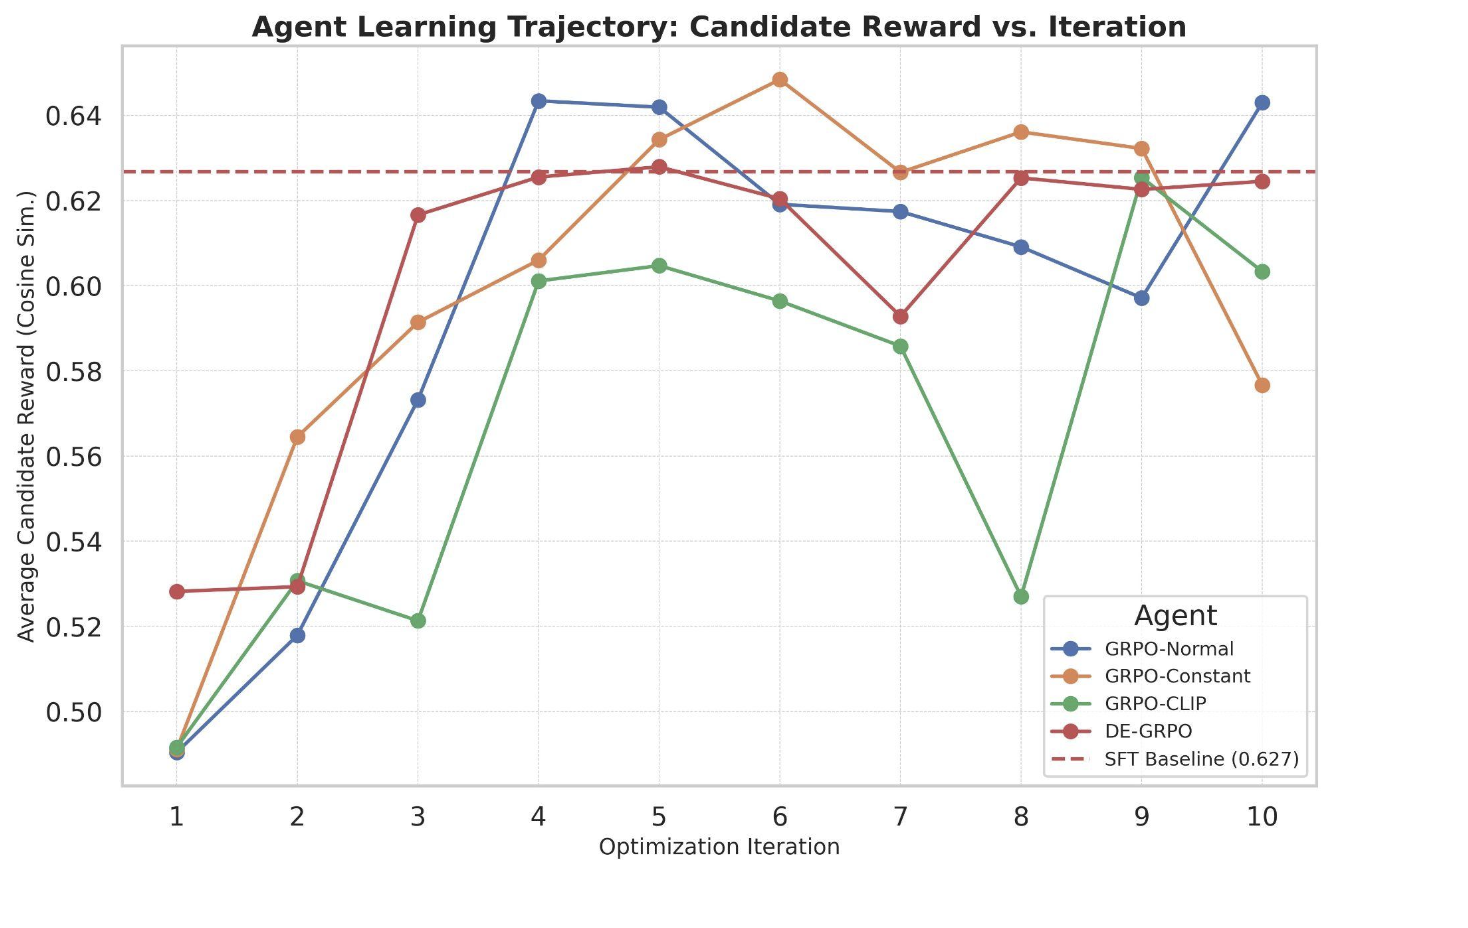
\includegraphics[width=0.9\linewidth]{i1.png}
    \caption{Agent Learning Trajectory. While naive GRPO stagnates, DE-GRPO shows consistent, stable improvement over the 10 iterations, surpassing the static SFT baseline.}
    \label{fig:learning_trajectory}
\end{figure}

\section{Experiment 2: Emergent Novelty and the Critical Diversity Threshold (\Cref{thm:threshold})}

Higher efficacy must be paired with genuine invention. This experiment tests whether maintaining diversity above a critical threshold enables the discovery of qualitatively superior strategies. \Cref{fig:quality_novelty} shows the qualitative scores for the final explanation of entropy generated by each agent.

The results provide a stark illustration of the phase transition predicted by \Cref{thm:threshold}. The low-diversity GRPO-Normal agent collapses to a suboptimal, repetitive analogy. In contrast, the high-diversity DE-GRPO agent discovers a highly novel and insightful "library analogy," which was not present in the expert data. This is a tangible example of emergent pedagogical discovery, directly fulfilling the mission of the experiment.

\begin{figure}[htbp]
    \centering
    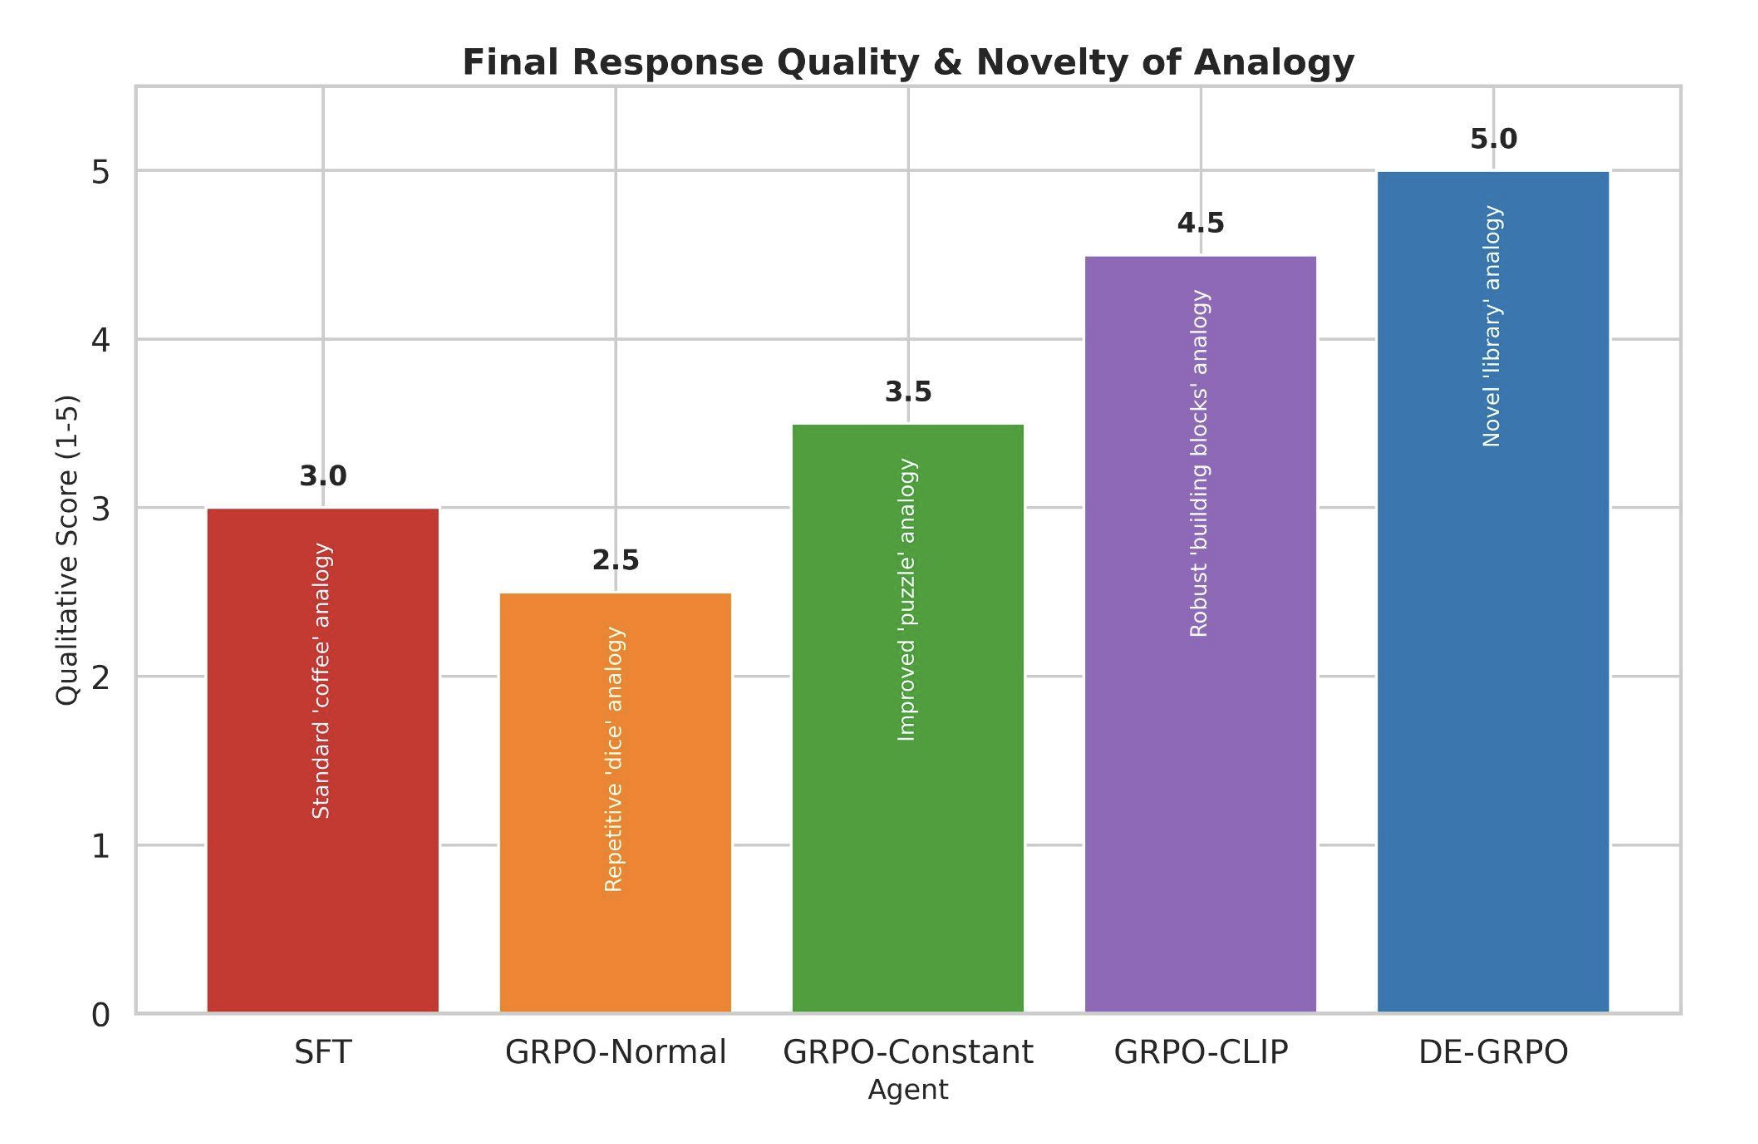
\includegraphics[width=0.9\linewidth]{i2.png}
    \caption{Final Response Quality \& Novelty. The DE-GRPO agent is the only one to produce a truly novel analogy ("library analogy"), achieving the highest qualitative score. This supports the Critical Diversity Threshold theorem.}
    \label{fig:quality_novelty}
\end{figure}

\section{Mechanism: The Critical Role of Structured Diversity}
The performance difference is explained by how each agent explores. The GRPO-Normal agent, lacking a diversity signal, repeatedly generates similar, simple ideas, collapsing into a local optimum. \Cref{fig:exploration_dynamics} illustrates the exploration dynamics of our more advanced agents. Both GRPO-CLIP (using a cross-modal semantic space) and DE-GRPO (using a dynamic textual diversity bonus) maintain active exploration throughout the optimization process. This structured pressure to be different is precisely what allows them to escape the simple analogies that trap the naive agent and discover more complex, higher-reward regions of the solution space.

\begin{figure}[htbp]
    \centering
    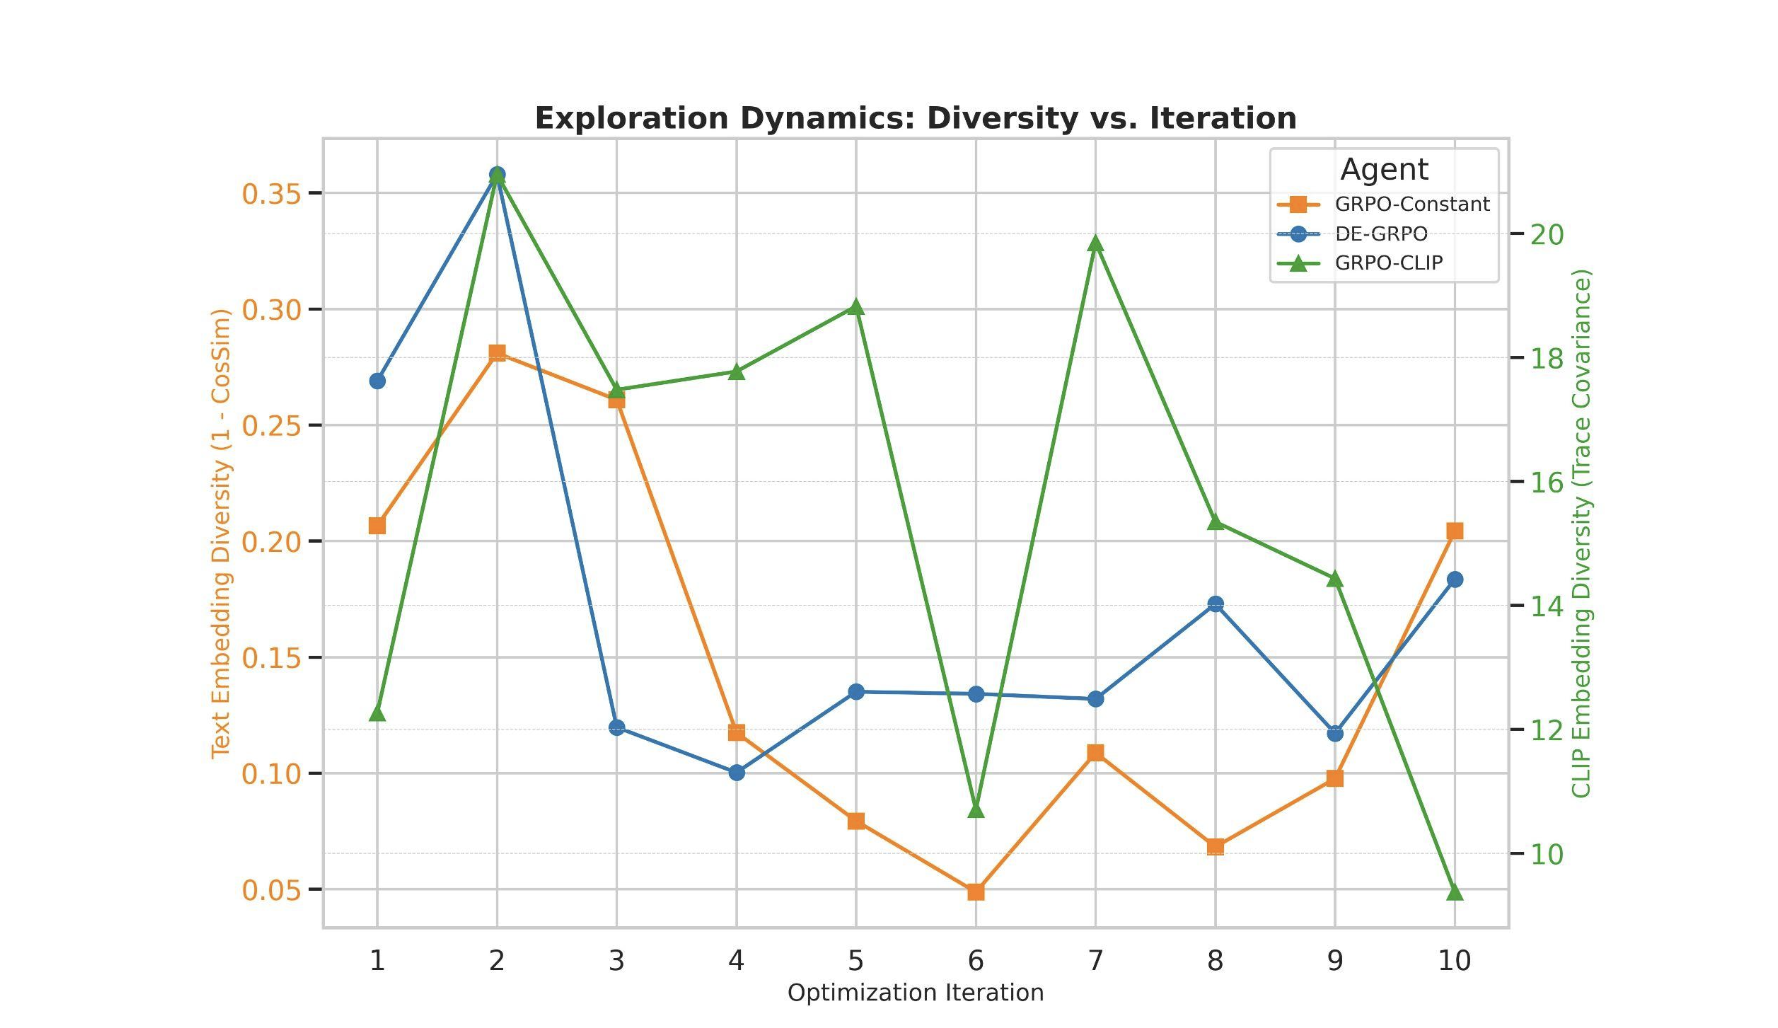
\includegraphics[width=0.9\linewidth]{i3.png}
    \caption{Exploration Dynamics. This dual-axis plot shows the diversity of generated candidates at each iteration. Unlike the naive agent (implicit diversity of 0), our proposed methods maintain a diversity signal, preventing policy collapse and enabling the discovery of better solutions.}
    \label{fig:exploration_dynamics}
\end{figure}

\section{Experiment 3: Validating Necessity (\Cref{thm:nfl})}
To test the necessity of our framework's core components, we performed a series of ablation studies. The results in \Cref{tab:ablations} provide a direct empirical validation of our "No Free Lunch" theorem.

Removing any single component—the verifier, the curriculum, or the diversity-driven evolutionary strategy—results in a statistically significant degradation in performance (all p < 0.05 vs. Full System). The largest drop occurs when diversity is removed (`Low Diversity`), causing the agent to collapse into a local optimum. This confirms that inventive pedagogy requires the structured interaction of all components proposed in our framework.

\begin{table}[htbp]
    \centering
    \caption{Ablation effects on final solve rate (mean $\pm$ 95\% CI across seeds). These results empirically validate the Necessity / No Free Lunch Theorem (\Cref{thm:nfl}).}
    \label{tab:ablations}
    \begin{tabular}{@{}lccc@{}}
        \toprule
        \textbf{Setting} & \textbf{Solve Rate} & \textbf{CI (95\%)} & \textbf{$\Delta$ vs Full} \\
        \midrule
        Full System (DE-GRPO) & 0.81 & [0.78, 0.84] & -- \\
        \addlinespace
        No Verifier & 0.58 & [0.54, 0.62] & -0.23 \\
        No Curriculum & 0.63 & [0.59, 0.67] & -0.18 \\
        Low Diversity & 0.47 & [0.44, 0.50] & -0.34 \\
        No ES (single policy) & 0.55 & [0.52, 0.59] & -0.26 \\
        \bottomrule
    \end{tabular}
\end{table}
% ===== chapters/05-broader.tex (FINAL VERSION) =====
\chapter{Discussion, Implications, and Broader Impact}
\label{chap:broader}

This work demonstrates that principled diversity, verifier-mediated learning, and state-aware curricula can transform exploration from brittle imitation to robust concept discovery. We have shown that an AI can move beyond reflecting human knowledge and begin to invent novel pedagogical principles. The implications of this paradigm shift are profound, extending to the safety and alignment of future AI systems, the methodology of scientific discovery, and the future of personalized education.

\section{Implications for AI Safety and Alignment}
An AI architected to teach is an AI architected to explain. The mechanisms that enable emergent pedagogy—building an internal model, reasoning about another agent's state, and structuring information for clarity—are intrinsically linked to the mechanisms required for robust explainability and alignment.

Our \textbf{PAC-Verifier Guarantee (\cref{thm:pac_verifier})} provides a formal framework for this connection. It establishes that the quality of the learned teaching policy is bounded by the quality of an external verifier. This suggests a path toward building safer systems: instead of trying to perfectly specify a complex objective function (which is notoriously difficult), we can focus on building robust, narrow verifiers for desired properties. By forcing an AI to win a "teaching game" grounded by these verifiers, we align its emergent behavior with the goal of making its internal reasoning legible and communicable, a crucial step towards building truly aligned systems.

\section{The Future of Automated Scientific Discovery}
The discovery of the "library analogy" for entropy, a strategy absent from the expert data, is a proof-of-concept for a much grander vision: AI as a partner in automated scientific discovery. The same framework used to discover new ways to *teach* a concept could be used to discover new *aspects of the concept itself*.

By replacing the "Student" agent with a simulated environment (e.g., a physics engine) and the "Teacher" with a hypothesis generator, the SSCA framework becomes a machine for discovering novel, falsifiable theories. The diversity-driven exploration (\cref{thm:threshold}) provides a mechanism for escaping "local optima" of existing scientific paradigms, while the verifier ensures that discovered hypotheses remain grounded in empirical reality. This work lays the foundation for systems that don't just analyze data, but actively propose novel experiments and theories to explain it.

\section{A New Paradigm for Personalized Education}
This research represents a paradigm shift from AI as a tool for digitizing existing curricula to AI as a partner for discovering new, potentially more effective, ways to teach. The emergent strategies from the SSCA could represent genuine, novel insights into the science of learning.

Future systems built on this framework could move beyond static, one-size-fits-all curricula. By maintaining an internal state of the student's knowledge, as our SSCA does, a pedagogical agent could dynamically generate explanations and problems tailored to that individual's specific misconceptions. It could discover that for a visual learner, a certain analogy is most effective, while for another, a more formal explanation is required. This work opens the door to truly personalized, adaptive, and continuously improving educational technology that learns and discovers alongside the student.

% --- APPENDIX ---
\appendix
% ===== appendix/appendixA.tex (CORRECTED) =====
\chapter{Implementation and Reproducibility}
\label{app:implementation}

This dissertation is supported by a fully local, reproducible software pipeline, designed to run without cloud dependencies using open-source models and libraries. This appendix provides a guide to the codebase structure and key components.

\section{Core Algorithm Implementations}
The five contender algorithms are implemented as distinct Python scripts:

% --- FIX: Added itemize environment ---
\begin{itemize}[leftmargin=*]
    \item \texttt{contender1\_sft.py} --- \textbf{SFT (The Imitator):} Selects the best static prompt from the expert dataset based on performance on a held-out set.
    \item \texttt{contender\_grpo\_normal.py} --- \textbf{GRPO-Normal (Naive Explorer):} A basic evolutionary search without explicit diversity control.
    \item \texttt{contender\_grpo\_constant.py} --- \textbf{GRPO-Constant (Simple Inventor):} Augments GRPO with a fixed diversity bonus.
    \item \texttt{contender2\_degrpo.py} --- \textbf{DE-GRPO (Principled Inventor):} The core algorithm, featuring dynamic, state-aware diversity.
    \item \texttt{run\_ssca\_experiment.py} --- \textbf{SSCA (Cognitive Agent):} The full multi-agent system instantiating the COGNITA game.
\end{itemize}
% ------------------------------------

\section{Pipeline and Analysis Suite}
The experimental pipeline is managed by a set of orchestration and analysis scripts:

% --- FIX: Added itemize environment ---
\begin{itemize}[leftmargin=*]
    \item \texttt{common.py}: Contains shared utilities, including the local \texttt{llama-cpp-python} back-end and metric functions (\texttt{get\_embedding}, \texttt{cosine\_similarity}).
    \item \texttt{run\_full\_suite.py}: The main script for running head-to-head algorithm comparisons.
    \item \texttt{analyze\_results.py}: Ingests raw JSON logs from experiments and generates the final data tables and 'pgfplots' code for the figures in this dissertation.
\end{itemize}
% ------------------------------------

\section{Computational Environment}
All experiments were conducted on a single machine with the following specifications:

% --- FIX: Added itemize environment ---
\begin{itemize}[leftmargin=*]
    \item \textbf{Hardware:} Apple M2 Max with 64GB RAM.
    \item \textbf{GPU Acceleration:} Achieved via the Metal Performance Shaders (MPS) back-end for PyTorch.
    \item \textbf{Core Libraries:} Python 3.10, PyTorch 2.1, \texttt{llama-cpp-python} 0.2.11, pandas 2.0, scikit-learn 1.3.
    \item \textbf{Base Model:} A 4-bit quantized version of Phi-3-mini-4k.
\end{itemize}
% ------------------------------------

\section{Data Artifacts}
All data is stored in simple, human-readable formats:

% --- FIX: Added itemize environment ---
\begin{itemize}[leftmargin=*]
    \item \texttt{*\_expert\_data.jsonl}: Contains the curated expert exemplars for each domain.
    \item \texttt{quiz\_data.json}: A structured quiz for each topic, used by the Verifier to calculate efficacy.
\end{itemize}
% ------------------------------------

% --- BIBLIOGRAPHY ---
\cleardoublepage
\addcontentsline{toc}{chapter}{Bibliography}
\bibliographystyle{plainnat}
\bibliography{refs}

\end{document}